% !TeX root = proposal.tex
\chapter{Recommending Privacy Settings for Generalized/Public IoT}\label{chapter:generalIoT}

In chapter~\ref{chapter:acceptability}, we have discussed what are the key factors affecting users to adopt IoT systems/devices, the privacy risks caused by inappropriate privacy disclosure and the difficulties that people have when manually configuring their privacy-setting for their IoT systems/devices. To alleviate similar burden of doing this in OSN/mobile areas, researchers have applied machine learning techniques to predict people’s location-privacy preferences, thereby automatically configuring their location-privacy settings. 
%But none similar research has been done in IoT domain yet. 
Therefore, we speculate that machine learning algorithm based user clustering can also be used to recommend privacy-setting for IoT users.

In this chapter, we demonstrate our work completed in exploring recommending privacy settings for general IoT, including the dataset that we use, our methodology, the inspection of users' behaviors using statistical analyses, prediction of users' behaviors using machine learning techniques, and the privacy-setting prototypes that we create based on both statistical and machine learning results.

In this chapter the following questions will be answered:
\begin{itemize}
	\item Q1: What are the key parameters affecting the users' privacy decisions in a general IoT scenario?
	\item Q2: Can you cluster users of general IoT and provide them effective and accurate smart default/profiles of privacy-settings using machine learning techniques?
\end{itemize}

As we have already discussed, there is similarity in people’s privacy preferences. Therefore,
neighbourhood-based recommendations may be as accurate as model-based recommendations.
Furthermore, neighbourhood-based recommendations are made from crowdsourcing sources,
which means that their performance may be better than that of model-based recommenders when
the data of individual users are insufficient.

\section{Dataset and design}
As we have discussed in Chapter \ref{chapter:intro}, the development of usable privacy interfaces commonly relies on user studies with existing systems. Since the Intel control framework has yet to be implemented~\cite{chow2015hci}, this method is not possible. We therefore we leveraged data collected by Lee and Kobsa~\cite{lee2016understanding}, which asked 200 participants about their intention to allow or reject the IoT features presented in 14 randomized scenarios. They varied the scenarios in a mixed fractional factorial design along the following dimensions: `Who', `What', `Where', `Reason', and `Persistence' (See Table~\ref{tab:parameter}). A total of 2800 scenarios were presented to 200 participants (100 male, 99 female, 1 undisclosed) through Amazon Mechanical Turk. Four participants were aged between 18 and 20, 75 aged 20--30, 68 aged 30--40, 31 aged 40--50, 20 aged 50--60, and 2 aged $>$ 60.

For every scenario, participants were asked a total of 9 questions. Our study focuses on the \textbf{allow/reject} question: ``If you had a choice to allow/reject this, what would you choose?'', with options ``I would allow it'' and ``I would reject it''. We also used participants' answers to three attitudinal questions regarding the scenario:
\begin{itemize}
	\item \textbf{Risk:} How risky or safe is this situation? (7pt scale from ``very risky'' to ``very safe'')
	\item \textbf{Comfort:} How comfortable or uncomfortable do you feel about this situation? (7pt scale)
	\item \textbf{Appropriateness:} How appropriate do you consider this situation? (7pt scale)
\end{itemize}

\begin{table*}
	\caption{Parameters used in the experiment. Example scenarios: \\\emph{``A device of a friend records your video to detect your presence. This happens continuously, while you are at someone else's place, for your safety.''}\\\emph{``A government device reads your phone ID to detect your identity. This happens once, while you are in a public place (e.g. on the street), for health-related purposes.''}}
	\label{tab:parameter}
	\begin{tabular}{l | l}
		\hline
		\textbf{Parameter} & \textbf{Levels} 	 \\ \hline
		\multirow{7}{9.5em}{Who\\\rule{0pt}{4ex}\emph{The entity collecting the data}}		& 1. Unknown \\
		& 2. Colleague							 \\
		& 3. Friend								 \\
		& 4. Own device							 \\
		& 5. Business 							 \\
		& 6. Employer 							 \\
		& 7. Government							 \\ \hline
		\multirow{24}{9.5em}{What\\\rule{0pt}{4ex}\emph{The type of data collected and (optionally) the knowledge extracted from this data}}	& 1. PhoneID	\\	
		& 2. PhoneID$>$identity				\\	
		& 3. Location						\\	
		& 4. Location$>$presence			\\	
		& 5. Voice							\\	
		& 6. Voice$>$gender					\\	
		& 7. Voice$>$ age 					\\	
		& 8. Voice$>$identity				\\	
		& 9. Voice$>$presence				\\	
		& 10. Voice$>$mood					\\	
		& 11. Photo							\\	
		& 12. Photo$>$gender				\\	
		& 13. Photo$>$age  \\
		& 14. Photo$>$identity	 \\
		& 15. Photo$>$presence 	 \\
		& 16. Photo$>$mood 	 \\
		& 17. Video	 \\
		& 18. Video$>$gender	 \\
		& 19. Video$>$age 		 \\
		& 20. Video$>$presence 	 \\
		& 21. Video$>$mood 	 \\
		& 22. Video$>$looking at	 \\
		& 23. Gaze	 \\
		& 24. Gaze$>$looking at	 \\ \hline
		\multirow{4}{9.5em}{Where\\\rule{0pt}{4ex}\emph{The location of the data collection}}	& 1. Your place		\\
		& 2. Someone else's place		\\				
		& 3. Semi-public place (e.g. restaurant) \\
		& 4. Public space (e.g. street) \\ \hline
		\multirow{6}{9.5em}{Reason\\\rule{0pt}{4ex}\emph{The reason for collecting this data}} & 1. Safety	\\
		& 2. Commercial						\\
		& 3. Social-related	\\
		& 4. Convenience \\
		& 5. Health-related \\
		& 6. None \\ \hline
		\multirow{2}{9.5em}{Persistence} & 1. Once \\
		& 2. Continuously \\ 
		\emph{Whether data is collected once or continuously} & \\ \hline
	\end{tabular}
\end{table*}

We use this dataset in two phases. In our first phase, we develop a ``layered'' settings interface, where users make a decision on a less granular level (e.g., whether a certain recipient is allowed to collect their personal information or not), and only move to a more granular decision (e.g., what types of information this recipient is allowed to collect) when they desire more detailed control. This reduces the complexity of the decisions users have to make, without reducing the amount of control available to them. We use statistical analysis of the Lee and Kobsa dataset to decide which aspect should be presented at the highest layer of our IoT privacy-setting interface, and which aspects are relegated to subsequently lower layers.

In our second phase, we develop a ``smart'' default setting, which preempts the need for many users to manually change their settings~\cite{smith2013choice}. However, since people differ extensively in their privacy preferences~\cite{olson2005study}, it is not possible to achieve an optimal default that is the same for everyone. Instead, different people may require different settings. Outside the field of IoT, researchers have been able to establish distinct clusters or ``profiles'' based on user behavioral data~\cite{knijnenburg2013dimensionality, olson2005study, wisniewski2017making}. We perform machine learning analysis on this dataset to create a similar set of ``smart profiles'' for our general IoT privacy-setting interface.

\section{Statistical Analysis}\label{sec:sa1}

%
%In this section we analyze how users' behavioral intentions to allow or reject the information collection described in the scenario are influenced by the scenario parameters. In line with classic attitude-behavior models~\cite{ajzen1977attitude}, we also investigate whether users' attitudes regarding the scenario---their judgment of risk, comfort, and appropriateness---mediate these effects. This mediation analysis~\cite{baron1986moderator} involves the following test:
%\begin{itemize}
%\item \textbf{Test 1:} The effect of the scenario parameters (who, what, where, reason, persistence) on participants' attitudes (risk, comfort, appropriateness).
%\item \textbf{Test 2:} The effect of participants' attitudes on their behavioral intentions (the allow/reject decision).
%\item \textbf{Test 3:}  The effect of the parameters on behavioral intentions, controlling for attitudes.
%\end{itemize}
%
%If tests 1 and 2 are significant, and test 3 reveals a substantial reduction in conditional direct effect (compared to the marginal effect), then we can say that the effects of the scenario parameters on participants' behavioral intention are mediated by their attitudes. Moreover, if the conditional direct effect is (close to) zero, then the effects are fully (rather than partially) mediated.
%
%\subsection{Scenario Parameters and Attitude}\label{subsec:attitude}
%\subsubsection{ANOVA Test of Main Effects}
%To understand the effect of the scenario parameters on participants' attitudes, we created a separate \textit{linear mixed effects regression} (\textit{lmer}) model with a random intercept (to account for repeated measures on the same participant) for each dependent variable (risk, comfort, appropriateness), using the scenario parameters as independent variables. We employed a forward stepwise procedure, adding the strongest remaining parameter into the model at each step and comparing it against the previous model. Table~\ref{tab:anovaEffect} shows that all parameters except \textbf{where} have a significant effect on each of the attitudes.
%
%\subsubsection{Post-hoc Comparisons}
%We also conducted Tukey post hoc analyses to better understand how the various values of each parameter influenced the attitudes. \textbf{Where} was excluded from these analyses, as it did not have an overall significant effect. Some key findings of these post hoc analyses are:
%
%\begin{table}
%\centering
%\caption{Effect of scenario on attitudes. Each model builds upon and is tested against the previous.}
%\label{tab:anovaEffect}
%\begin{tabular}{ l | r | r | r}
%\hline
%Model &	$\chi^2$ &	$df$ & $p$-value \\ \hline
%$risk\sim(1|sid)$ &				 &			 &						\\
%+who &				315.37 &	6 &			$<$ .0001 		\\
%+what &			67.74 &		23 &		$<$ .0001 		\\
%+reason & 			15.65 &		5 &		.0079 			\\
%+persistence &		9.95 &		1 &		.0016 			\\
%+where	&			7.47 &		3 &		.0586 			\\
%+who:what &		166.47 &	138 &	.0050			\\
%\hline
%Model &	$\chi^2$ &	$df$ & $p$-value \\ \hline
%$comfort\sim(1|sid)$ & 			 &			&	 					\\
%+who &				334.06 &	6 &			$<$ .0001 		\\
%+what &			83.24 &		23 &		$<$ .0001 		\\
%+reason &			18.68 &		5 &			.0022 		\\
%+persistence &		14.73 &		1 &			.0001 		\\
%+where &			3.25 &		3 &			.3544 		\\
%+who:what &		195.07 &	138 &		.0001			\\
%\hline
%Model &	$\chi^2$ &	$df$ & $p$-value \\ \hline
%$appropriateness\sim(1|sid)$ &	 &		 &						\\
%+who &				315.77 &	6 &			$<$ .0001 		\\
%+what &			72.87 &		23 &		$<$ .0001 		\\
%+reason &			23.27 &		5 &			.0003 		\\
%+persistence &		8.97 &		1 &			.0027 		\\
%+where &			5.46 &		3 &			.1411 		\\
%+who:what &		214.61 &	138 &		$<$ .0001			\\
%\hline
%\end{tabular}
%\end{table}
%
%\textbf{Who:} Participants perceive more \emph{risk} when the recipient of the information is `unknown' than for any other recipient ($d$ range = [0.640, 1.450] and all $p$s~$<$~.001, except for `government': $d=0.286$, $p < .05$). `Government' is the next most risky recipient ($d$ range = [0.440, 1.190], all $p$s~$<$~.001). Participants consider their `own device' the least risky ($d$ range = [0.510, 1.450], all $p$s~$<$~.001). Similar patterns were found for \emph{comfort} and \emph{appropriateness}.
%
%\textbf{Reason:} Participants were more \emph{comfortable} disclosing information for the purpose of `safety' than for any other reason except `health' ($d$ range = [0.230, 0.355], all $p$s~$<$~.05). They also believe that disclosing information for the purpose of `health' or `safety' is more \emph{appropriate} than for `social' or `commercial' purposes ($d$ range = [0.270, 0.310], all $p$s~$<$~.05).
%
%\textbf{Persistence:} Participants were more \emph{comfortable}, found it more \emph{appropriate}, and less \emph{risky} to disclose their information `once' rather than `continuously' ($d = 0.146$, $p < .01$).
%
%\textbf{What:} This parameter has a large number of values, so we decided to selectively test planned contrasts instead of post-hoc tests. We first compared different mediums (voice, photo, video) regardless of what is being inferred:
%\begin{itemize}
%\item Participants were significantly more \emph{comfortable} with `voice' than `video' ($d = 0.260$, $p = .005$), and found `voice' less \emph{risky} ($d = -0.239$, $p = .005$) and more \emph{appropriate} ($d = 0.217$, $p = .015$) than `video'.
%\item Participants were significantly more \emph{comfortable} with `voice' than `photo' ($d=0.201$, $p = .007$) and found `voice' more \emph{appropriate} than `photo' ($d = 0.157$, $p$~$=$~$.028$). There was no significant difference in terms of \emph{risk} ($p = .118$).
%\item No differences were found between `photo' and `video' in terms of \emph{risk} ($p = .24$), \emph{comfort} ($p = .35$) and \emph{appropriateness} ($p = .26$).
%\end{itemize}
%
%We also compared different inferences (e.g. age, gender, mood, identity) across mediums. The following planned contrasts were significant (all others were not):
%\begin{itemize}
%\item Participants were significantly more \emph{comfortable} ($d$~$=$~$0.363$, $p = .028$) and found it more \emph{appropriate} ($d = 0.371$, $p = .018$) to reveal their `age' rather than their `identity'.
%\item Participants were significantly more \emph{comfortable} ($d$~$=$~$0.363$, $p= .008$) and found it more \emph{appropriate} ($d = 0.308$, $p = .024$) to reveal their `presence' rather than their `identity'.
%\end{itemize}
%
%\subsubsection{Interaction effects}
%We also checked for two-way interactions between the scenario parameters. The only significant interaction effect observed was between \textbf{who} and \textbf{what}. The last line of each section in Table~\ref{tab:anovaEffect} shows the results of adding this interaction to the model. Due to space concerns, we choose not to address the post-hoc analysis of the $7 * 24 = 168$ specific combinations of who and what.
%
%\subsection{Attitude and Behavioral intention}
%To test the effects of participants' attitudes on their allow/reject decision, we ran a \emph{generalized linear mixed effects regression} (\emph{glmer}) with a random intercept and a logit link function to account for the binary dependent variable.
%We found significant effects of all the three attitudes on participants' allow/reject decision (see Table~\ref{tab:mediationANOVA}). Each 1-point increase in \textbf{risk} results in a 4.04-fold decrease in the odds that the scenario will be allowed ($p < .0001$). Each 1-point increase in \textbf{comfort} results in a 5.04-fold increase ($p < .0001$), and each 1-point increase in \textbf{appropriateness} results in a 3.47-fold increase ($p < .0001$).
%
%\subsection{Mediation Analysis}
%The bottom half of Table~\ref{tab:mediationANOVA} shows the \emph{conditional} effects of the significant parameters (who, what, reason, persistance) on participants' allow/reject decision, controlling for attitude. \textbf{Who} and \textbf{what} are no longer significant; these effects are thus fully mediated by attitude. The effects of \textbf{reason} and \textbf{persistance} are still significant, but smaller than the marginal effects (i.e., without controlling for attitude, see Table~\ref{tab:marginalANOVA})---their $\chi^2$s are reduced by 12\% and 39\%, respectively. This means that the mediation effect was substantial in all cases. The final mediation model is displayed in Figure~\ref{fig:mediationAllow}.
%
%
%\begin{table}
%\centering
%\caption{Effect of attitudes and scenario on allow/reject.}
%\label{tab:mediationANOVA}
%\begin{tabular}{ l | r | r | r | r }
%\hline
%Model & OR	&	\textbf{$\chi^2$} & $df$ & $p$-value 	\\ \hline
%$allow\sim(1 | sid)$ &	&		  &	    &				\\
%+risk &				0.25 &	1005.24  &    1 &		$<$ .0001 \\
%+comfort &			5.04 &	723.27  &     1 &		$<$ .0001 \\
%+appropriateness &	3.47 &	128.17  &	  1 & 		$<$ .0001 \\ \hline
%+who &					&	8.80	& 	  6 & 		.1851 	\\
%+what &					&	26.07 &	  	 23 &		.2976 	\\
%+reason &				&	19.33 & 	  5 & 		.0017	\\
%+persistence &			&	12.69 &	 	  1 & 		.0004 	\\
%\hline
%\end{tabular}
%\end{table}
%
%\begin{table}
%\centering
%\caption{Effect of scenario on allow/reject, \emph{not} controlling for attitudes.}
%\label{tab:marginalANOVA}
%\begin{tabular}{ l | r | r | r }
%\hline
%Model &	$\chi^2$ & $df$ & $p$-value 	\\ \hline
%$allow\sim(1 | sid)$ &		  	&	    &				\\
%+who &					221.36	& 	  6 & 		$<$ .0001 	\\
%+what &					78.55 &		  23 &		$<$ .0001 	\\
%+reason &				21.95 & 	  5 & 		  .0005		\\
%+persistence &			20.64 &		  1 & 		$<$ .0001 	\\
%\hline
%\end{tabular}
%\end{table}
%
%\begin{figure}
%\centering
%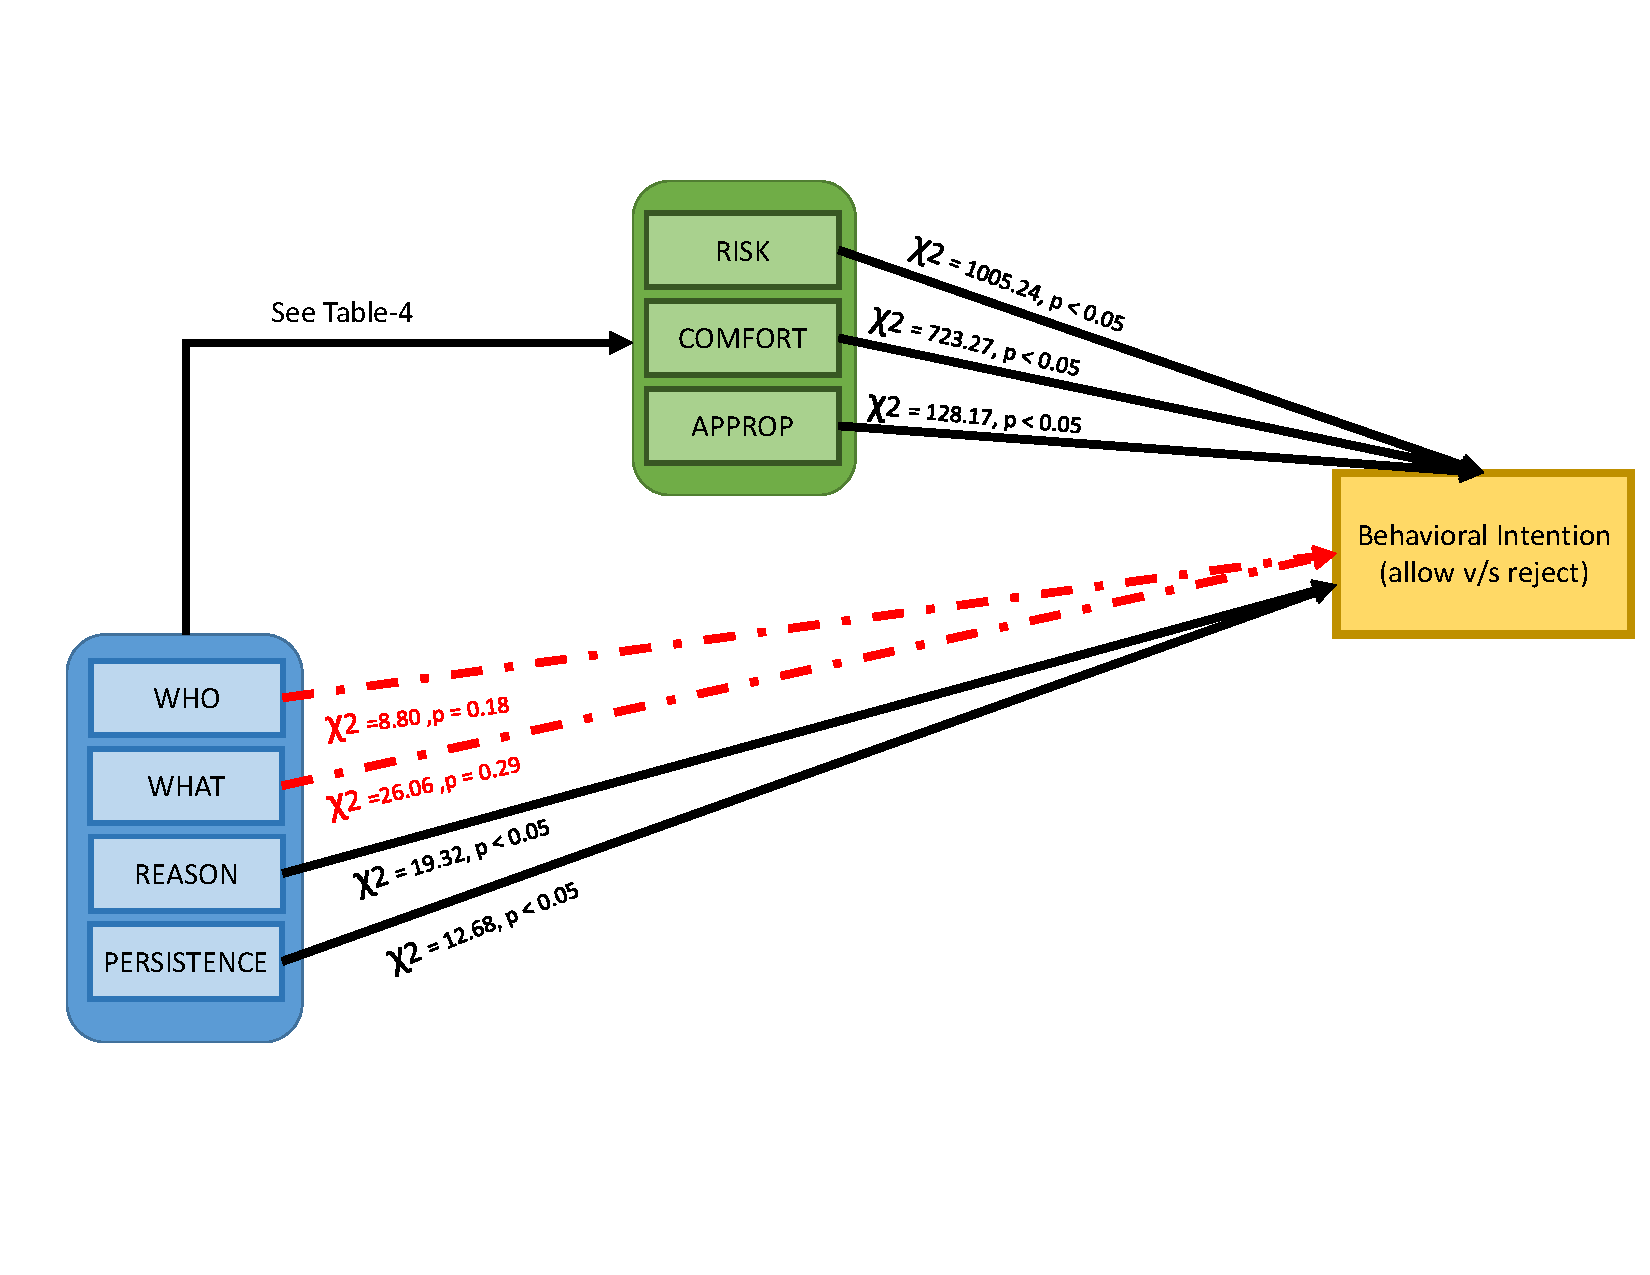
\includegraphics[width=0.45\textwidth]{figures/allow.pdf}
%\caption{Mediation model of the effect of scenario parameters on participants' intention to allow/reject the scenario, mediated by attitudinal factors}
%\label{fig:mediationAllow}
%\end{figure}

%\subsection{Discussion of Statistical Results}
We conducted a statistical analysis on this dataset to determine the effect of each scenario parameter on users' decisions to allow the presented general IoT scenario and how this effect is mediated by the user's attitudes. \footnote{The statistical analysis and the subsequent layered interface were developed by my co-author Paritosh Bahirat. These endeavors are presented in summarized form since they are not an official part of this dissertation. For more details, please refer to~\cite{bahiratiui2018}.}

Using this approach, we find that the `Who' parameter has the strongest effect on users' decision to allow the scenario, followed by the `What', the `Reason', and the 'Persistence' parameter. The `Where' parameter has no effect at all. People are generally concerned about IoT scenarios involving unknown and government devices, but less concerned about about data collected by their own devices. Mistrust of government data collection is in line with Li et al.'s finding regarding US audiences~\cite{li2017cross}.

`What' is the second most important scenario parameter, and its significant interaction with `who' suggests that some users may want to allow/reject the collection of different types of data by different types of recipients. Privacy concerns are higher for photo and video than for voice, arguably because photos and videos are more likely to reveal the identity of a person. Moreover, people are less concerned with revealing their age and presence, and most concerned with revealing their identity.

The `reason' for the data collection is the third most important scenario parameter. Health and safety are generally seen as acceptable reasons. `Persistence' is less important, although one-time collection is more acceptable than continuous collection. `Where' the data is being collected does not influence intention at all. This could be an artifact of the dataset: location is arguably less prominent when reading a scenario than it is in real life.

Finally, participants' attitudes significantly (and in some cases fully) mediated the effect of scenario parameters on behavioral intentions. This means that these attitudes may be used as a valuable source for classifying people into distinct groups. Such attitudinal clustering could capture a significant amount of the variation in participants in terms of their preferred privacy settings, especially with respect to the `who' and `what' dimensions.

Moreover, we found no significant interaction effects of parameters on decision. The only significant interaction however was between `Who' and `What' onto the attitudes. The outcome informed the design of a `layered interface', which present privacy settings with the most prominent influence first, relegating less prominent aspects to subsequently lower layers (See Figure~\ref{fig:interface1}). Users can make a decision based on a single parameter only, and choose `yes', `no', or `it depends' for each parameter value. If they choose `it depends', they move to a next layer, where the decision for that parameter value is broken down by another parameter.

The manual interface is shown in Screens 2-4 of Figure~\ref{fig:interface1}. At the top layer of this interface should be the scenario parameter that is most influential in our dataset. Our statistical results inform us that this is the \textbf{who} parameter. Screen 2 shows how users can allow/reject data collection for each of the 7 types of recipients. Users can choose ``more'', which brings them to the second-most important scenario parameter, i.e. the \textbf{what} parameter. Screen 3 of Figure~\ref{fig:interface1} shows the data type options for when the user clicks on ``more'' for ``Friends' devices''. We have conveniently grouped the options by collection medium. Users can turn the collection of various data types by their friends' devices on or off. If only some types of data are allowed, the toggle at the higher level gets a yellow color and turns to a middle option, indicating that it is not completely `on' (see ``Friends' devices'' in Screen 2).

Screen 4 of Figure~\ref{fig:interface1} shows how users can drill down even further to specify \textbf{reasons} for which collection is allowed, and the allowed \textbf{persistence} (we combined these two parameters in a single screen to reduce the ``depth'' of our interface). Since \textbf{reason} and \textbf{persistence} explain relatively little variance in behavioral intention, we expect that only a few users will go this deep into the interface for a small number of their settings. We leave out \textbf{where} altogether, because our statistical results deemed this parameter to be non-significant.

\begin{figure}
	\centering
	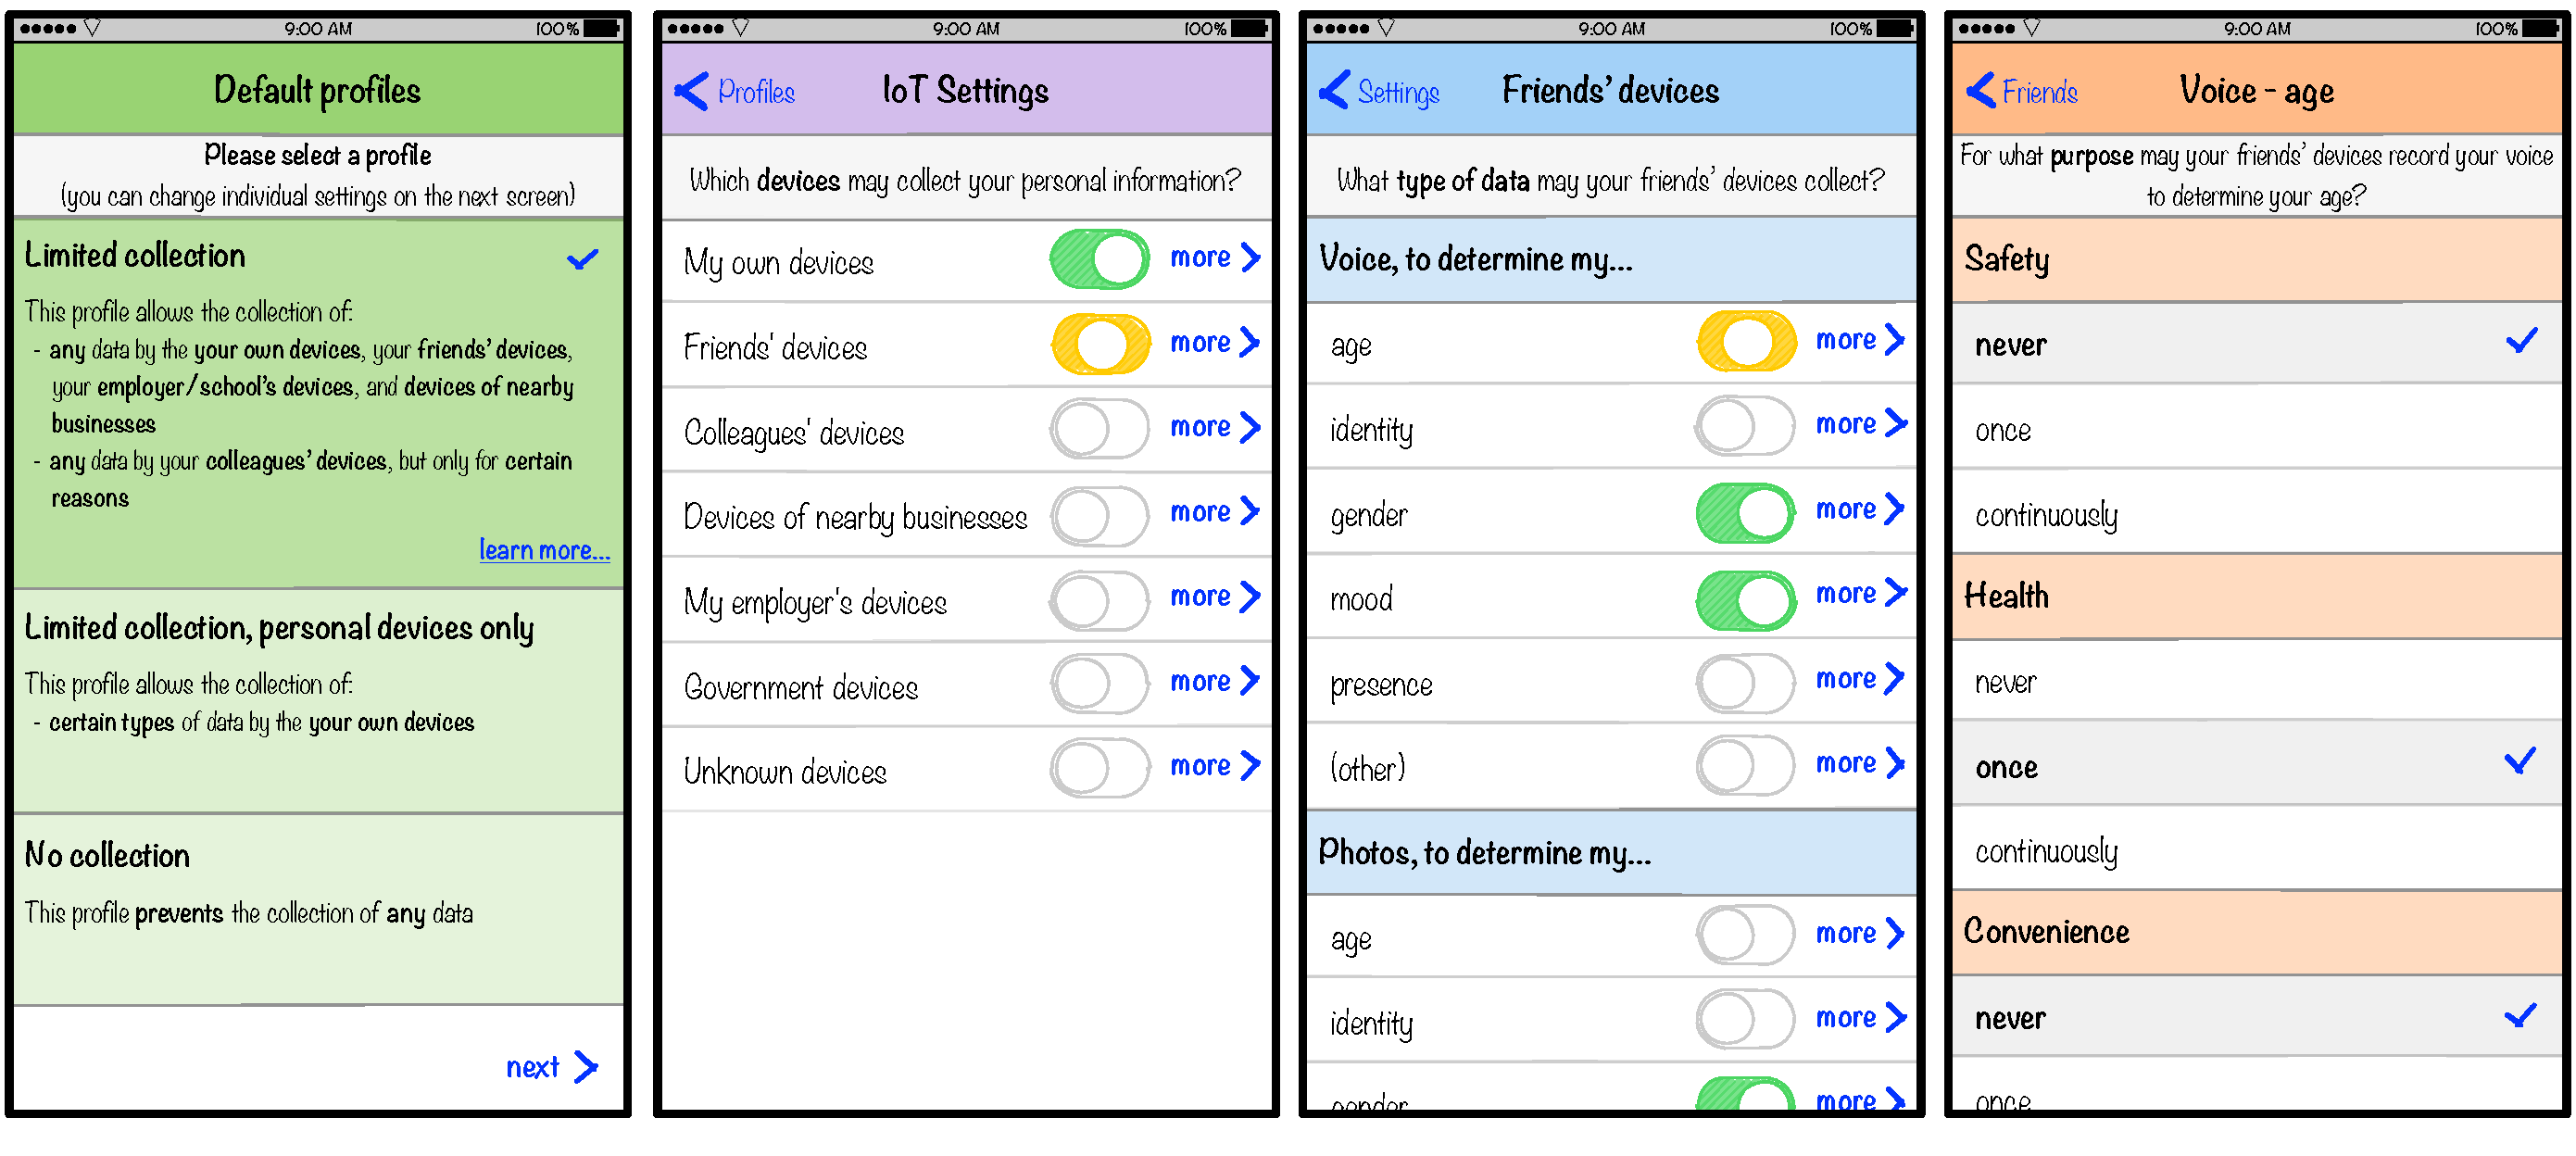
\includegraphics[width=0.8\textwidth]{figures/interface1.pdf}
	\caption{From Left, Screen 1 shows three default settings, Screen 2,3 and 4 shows layered interface}
	\label{fig:interface1}
\end{figure}

\section{Predicting users' behaviors (original work)}\label{sec:predict1}
To further simplify the task of manually setting privacy preferences, we used machine learning to predict users' decisions based on the scenario parameters. Our goal is to find suitable \emph{default settings} for an IoT privacy-setting interface. Consequently, we do not attempt to find the most accurate solution; instead we make a conscious tradeoff between parsimony and prediction accuracy. Accuracy is important to ensure that users' privacy preferences are accurately captured and/or need only few manual adjustments. Parsimony, on the other hand, prevents overfitting and promotes fairness: we noticed that more complex models tended to increase overall accuracy by predicting a few users' preferences more accurately, with no effect on other users. Parsimony also makes the associated default setting easier to understand for the user. 

Our prediction target is the participants' decision to allow or reject the data collection described in each scenario, classifying a scenario as either `yes' or `no'. The scenario parameters serve as input attributes. These are nominal variables, making decision tree algorithms such as ID3 and J48 a suitable prediction approach. Unlike ID3, J48 uses gain ratio as the root node selection metric, which is not biased towards input attributes with many values. We therefore use J48 throughout our analysis.

We discuss progressively sophisticated methods for predicting participants' decisions. After discussing naive solutions, we first present a cross-validated tree learning solution that results in a single ``smart default'' setting that is the same for everyone. Subsequently, we discuss three different procedures that create a number of ``smart profiles'' by clustering the participants and creating a separate cross-validated tree for each cluster. For each procedure, we try various numbers of clusters. Accuracies of the resulting solutions are reported in Table~\ref{tab:comp_approach}.

\subsection{Naive Prediction Methods}
We start with naive or ``information-less'' predictions. Our dataset contains 793 `yes'es and 2007 `no's. Therefore, predicting `yes' for every scenario gives us a 28.33\% prediction accuracy, while making a `no' prediction gives us an accuracy of 71.67\%. In other words, if we disallow all information collection by default, users will on average be happy with this default for 71.67\% of the settings.



\begin{table}
	\centering
	\caption{Comparison of clustering approaches}
	\label{tab:comp_approach}
	\begin{tabular}{  l |  l |  l | l}
		\hline
		Approach & clusters & Accuracy & \# of profiles \\ \hline
		\multirow{2}{6em}{Naive classification} & 1 & 28.33\% & 1  (all `yes')\\ %\cline{2-4}
		& 1 & 71.67\% & 1 (all `no') \\ \hline
		Overall & 1 & 73.10\% & 1 \\ \hline 
		\multirow{4}{6em}{Attitude-based clustering} & 2 & 75.28\% & 2 \\ %\cline{2-4}
		& 3 & 75.17\% & 3 \\ %\cline{2-4}
		& 4 & 75.60\% & 3 \\ %\cline{2-4}
		& 5 & 75.25\% & 3 \\ \hline
		%	\multirow{3}{6em}{Trait-based Clustering} & 2 & 75.57\% & 2 \\ %\cline{2-4}
		%	& 3 & 75.10\% & 2 \\ %\cline{2-4}
		%	& 4 & 75.57\% & 2 \\ %\cline{2-4}
		%	& 5 & 75.07\% & 2 \\ \hline
		\multirow{2}{6em}{Fit-based clustering} & 2 & 77.99\% & 2 \\ %\cline{2-4}
		& 3 & 81.54\% & 3 \\ \hline
		\multirow{2}{6em}{Agglomerative  clustering} & 200 & 78.13\% & 4 \\ %\cline{2-4}
		& 200 & 78.27\% & 5 \\ \hline %\cline{2-4} 
	\end{tabular}
\end{table}

\subsection{Overall Prediction}
We next create a ``smart default'' by predicting the allow/reject decision with the scenario parameters using J48 with Weka's~\cite{hall2009weka} default settings. The resulting tree is shown in Figure~\ref{fig:naive_cls}). The confusion matrix (Table~\ref{tab:confusion_matrix}) shows that this model results in overly conservative settings; only 208 `yes'es are predicted.

\begin{table}
	\centering
	\caption{Confusion matrix for the overall prediction}
	\label{tab:confusion_matrix}
	\begin{tabular}{c|c|c|c} \hline
		Observed &\multicolumn{2}{c|}{Prediction} & Total\\ \cline{2-3}
		& Yes     & No       &  \\ \hline
		Yes   & 124 (TP) & 669 (FN)  & 793   \\ \hline
		No    & 84 (FP)  & 1923 (TN) & 2007  \\ \hline
		Total & 208     & 2592     & 2800  \\ \hline
	\end{tabular}
\end{table}

Figure~\ref{fig:naive_cls} shows that this model predicts `no' for every recipient (`who') except `Own device'. For this value, the default setting depends on `what' is being collected (see Table~\ref{tab:decisions}). For some levels of `what', there is a further drill down based on `where', `persistence' and `reason'.

We can use this tree to create a ``smart default'' setting; in that case, users would on average be content with 73.10\% of these settings---a 2\% improvement over the naive ``no to everything'' default setting. 

Given that people differ substantially in their privacy preferences, it is not unsurprising that this ``one size fits all'' default setting is not very accurate. A better solution would cluster participants by their privacy preferences, and then fit a separate tree for each cluster. These trees could then be used to create ``smart profiles'' that new users may choose from. Subsequent sections discuss several ways of creating such profiles.

\begin{figure}
	\centering
	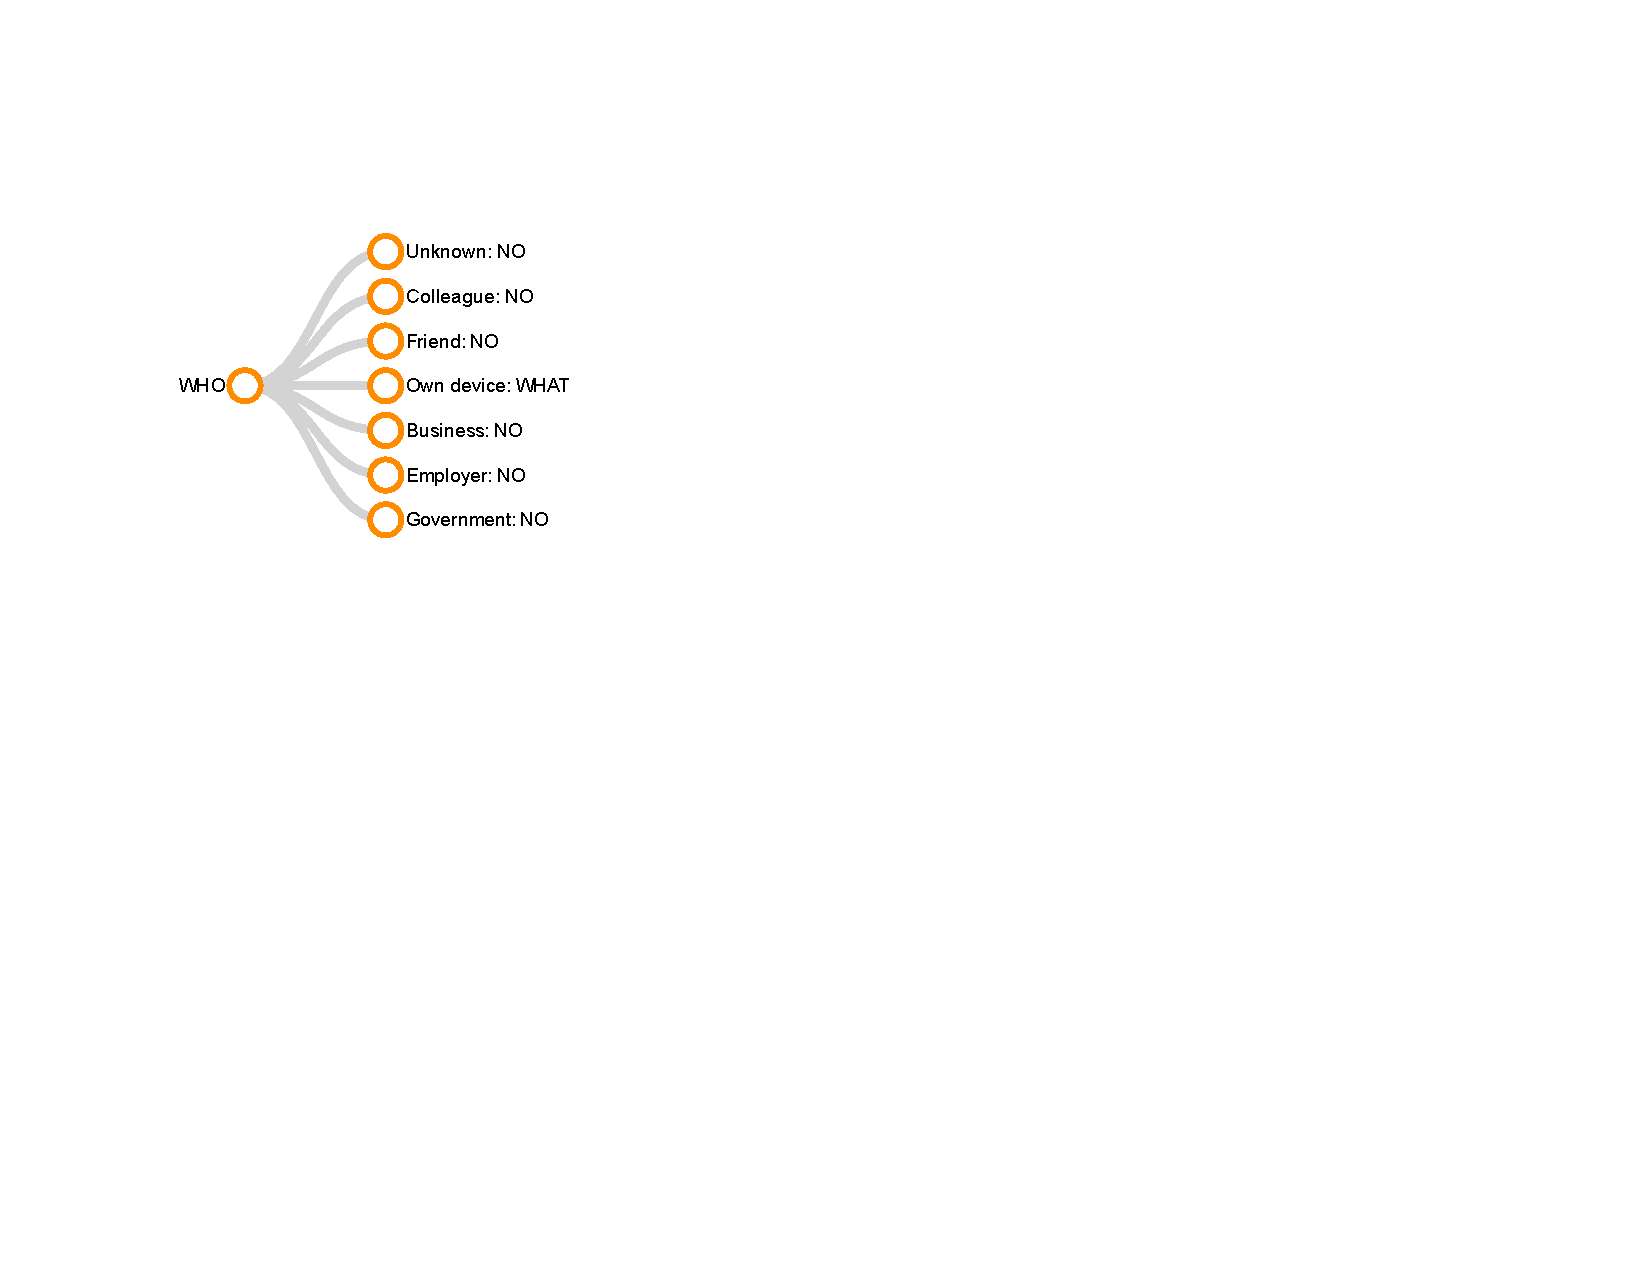
\includegraphics[width=.22\textwidth]{figures/overall.pdf}
	\caption{The Overall Prediction decision tree. Further drill down for `who' = `Own device' is provided in Table~\ref{tab:decisions}}
	\label{fig:naive_cls}
\end{figure}

\begin{table}
	\centering
	\caption{Drill down of the Overall Prediction tree for `who' = `Own device'}
	\label{tab:decisions}
	\begin{tabular}{ l | l }
		\hline
		\textbf{What} & \textbf{Decision} \\ \hline
		PhoneID				& Yes			\\
		PhoneID$>$identity 	& Yes			\\
		Location 			& No			\\
		Location$>$presence 	& Reason
		$\left\{
		\begin{tabular}{l | l}
		Safety & Yes \\ 
		Commercial & Yes \\
		Social-related & No \\
		Convenience & No \\
		Health-related & Yes \\
		None & Yes \\
		\end{tabular}\right.$ \\
		Voice 				& No			\\
		Voice$>$gender 		& Where 
		$\left\{
		\begin{tabular}{l | l}
		Your place & No\\
		Someone else & No \\
		Semi-public & No \\
		Public & Yes \\
		\end{tabular}\right.$ \\
		Voice$>$ age 			& No			\\
		Voice$>$identity 		& Yes			\\
		Voice$>$presence 		& Yes			\\
		Voice$>$mood 			& Yes			\\
		Photo 				& No			\\
		Photo$>$gender 		& No			\\
		Photo$>$age 			& No			\\
		Photo$>$identity 		& Yes			\\
		Photo$>$presence 		& No			\\
		Photo$>$mood 			& No			\\
		Video 				& No			\\
		Video$>$gender 		& No			\\
		Video$>$age 			& No			\\
		Video$>$presence 		& No			\\
		Video$>$mood 			& Yes			\\
		Video$>$looking at 	& Persistence
		$\left\{
		\begin{tabular}{l | l}
		Once & Yes \\
		Continuous & No \\
		\end{tabular}\right.$ \\
		Gaze 				& No			\\
		Gaze$>$looking at 	& Reason
		$\left\{
		\begin{tabular}{l | l}
		Safety & Yes \\
		Commercial & No \\
		Social-related & No \\
		Convenience & Yes \\
		Health-related & Yes \\
		None & Yes \\
		\end{tabular}\right.$ \\
	\end{tabular}
\end{table}


\subsection{Attitude-Based Clustering}
Our first ``smart profile'' solution uses the attitudes (comfort, risk, appropriateness) participants expressed for each scenario on a 7-point scale. We averaged the values per attitude across each participant's 14 answers, and ran $k$-means clustering on that data with 2, 3, 4 and 5 clusters. We then added participants' cluster assignments to our original dataset, and ran the J48 decision tree learner on the dataset with the additional \textbf{cluster} attribute. Accuracies of the resulting solutions are reported in Table~\ref{tab:comp_approach} under ``attitude-based clustering''.


All of the resulting trees had \textbf{cluster} as the root node. This indicates that this parameter is a very effective parameter for predicting users' decisions. This also allows us to split the trees at the root node, and create separate default settings for each cluster.

The 2-cluster solution (Figure~\ref{fig:2clusters}) has a 75.28\% accuracy --- a 3.0\% improvement over the ``smart default''. This solution results in one profile with `no' for everything, while for the other profile the decision depends on the recipient (\textbf{who}). This profile allows any collection involving the user's `Own device', and may allow collection by a `Friend' or an `Employer/School', depending on \textbf{what} is being collected.

\begin{figure}
	\centering
	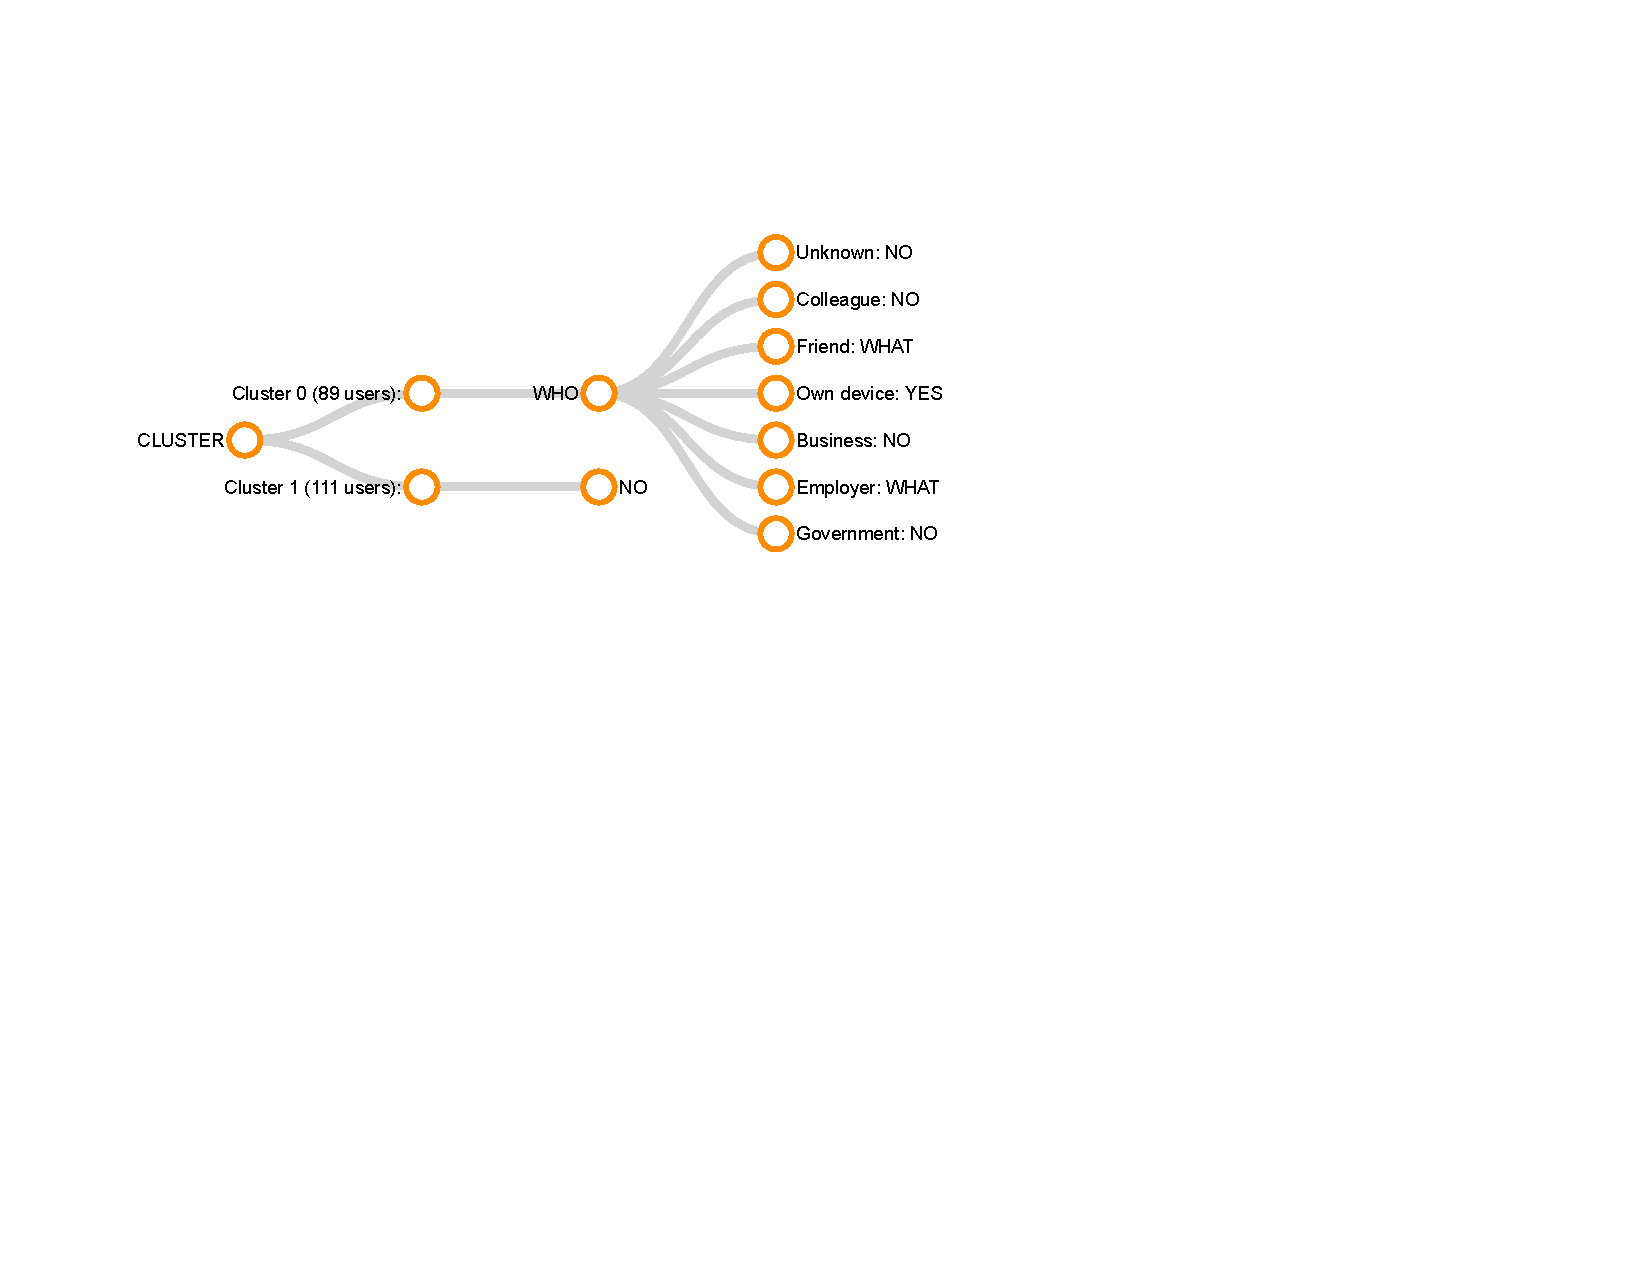
\includegraphics[width=0.8\textwidth]{figures/attitude-based-2.pdf}
	\caption{Attitude-based clustering: 2-cluster tree. Further drill down for \textbf{who} = `Friend' or `Employer/School' in Cluster 0 is hidden for space reasons.}
	\label{fig:2clusters}
\end{figure}

The 3-cluster solution has a slightly lower accuracy of 75.17\%, but is more parsimonious than the 2-cluster solution. There is one profile with `no' for everything, one profile that allows collection by the user's `Own device' only, and one profile that allows any collection except when the recipient is `Unknown' or the `Government'. The 4- and 5-cluster solutions have several clusters with the same sub-tree, and therefore reduce to a 3-cluster solution with 75.60\% and 75.25\% accuracy, respectively.


\begin{figure}
	\centering
	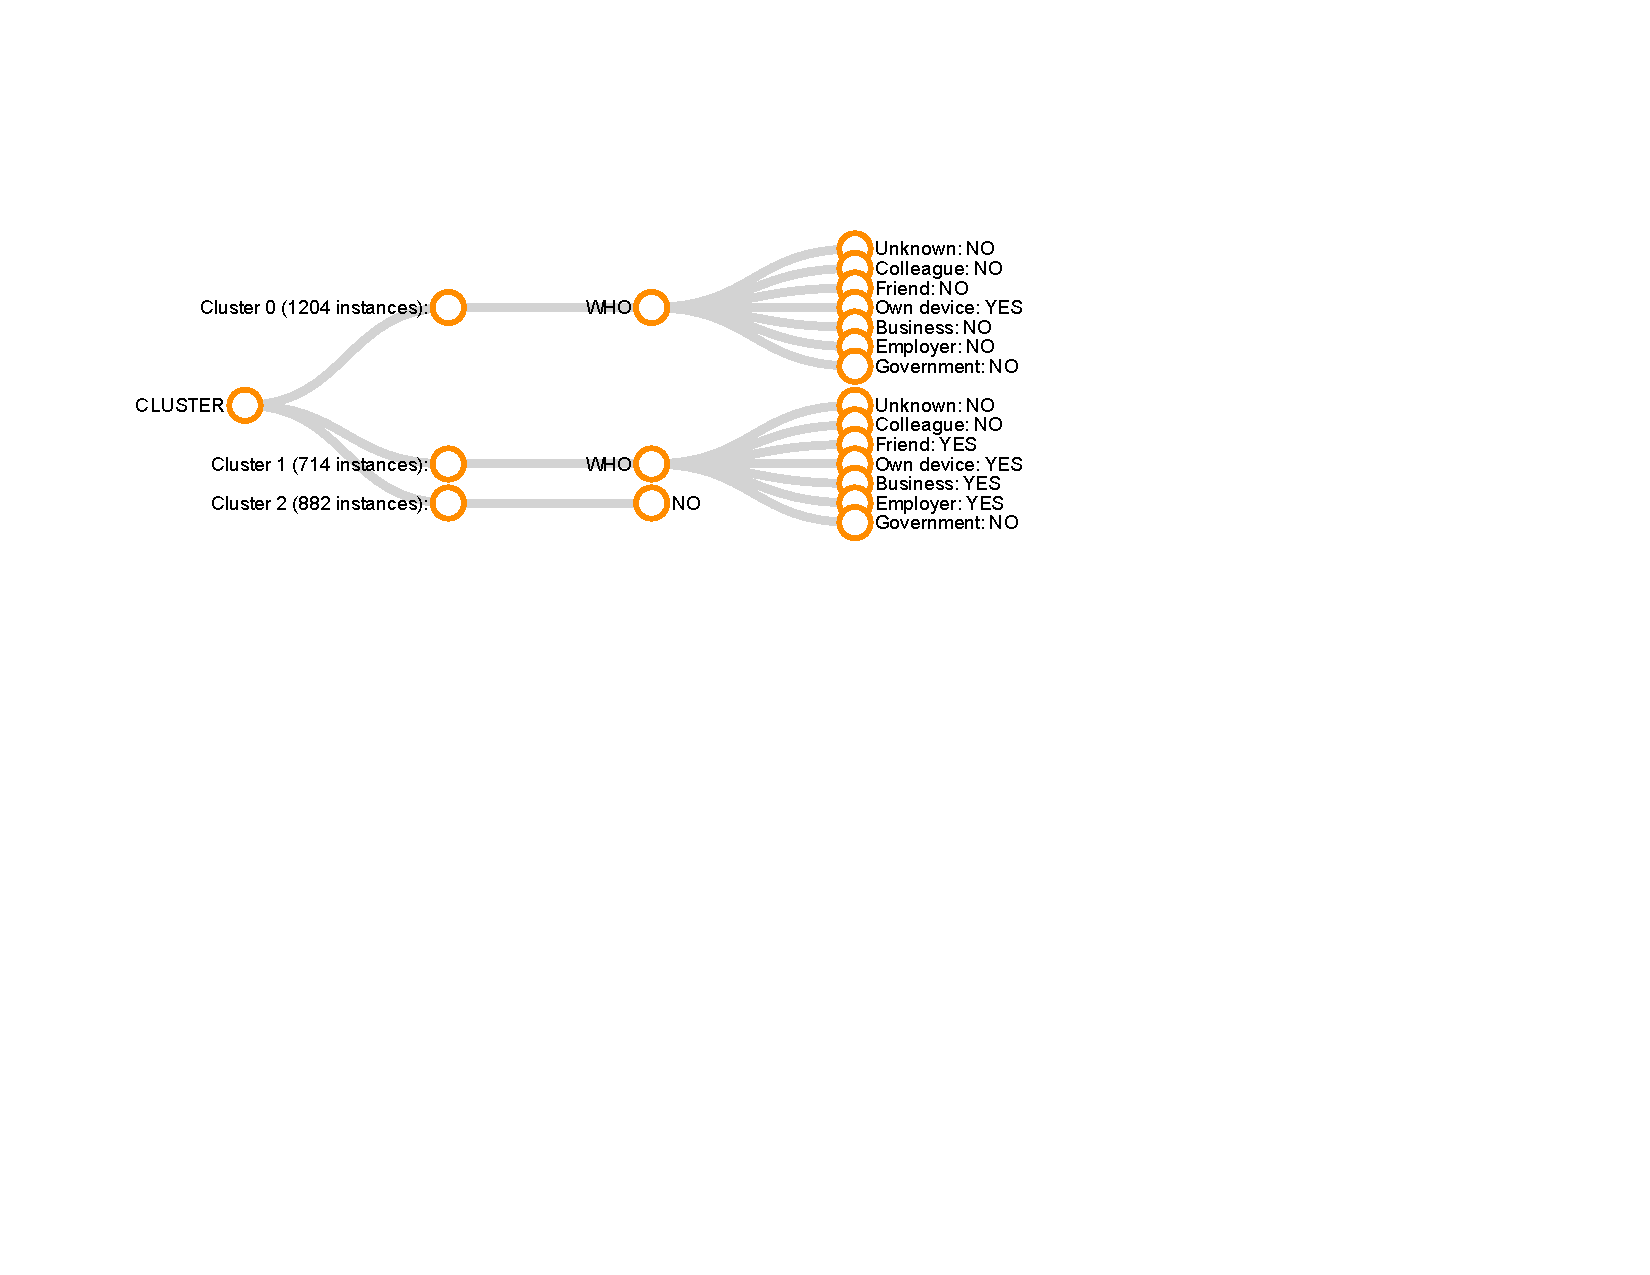
\includegraphics[width=0.8\textwidth]{figures/attitude-based-3.pdf}
	\caption{Attitude-based clustering: 3-cluster tree}
	\label{fig:3clusters}
\end{figure}


%\subsection{Trait-based clustering}
%Our second ``smart profile'' solution uses the 13 subjective questions asked towards the end of the survey conducted by Lee and Kobsa~\cite{lee2016understanding} regarding participants' privacy concerns, mobile Internet usage, and tech savviness. Confirmatory Factor Analysis was performed to extract latent traits from these questions, followed by a Factor Mixture Analysis to cluster participants on these traits into 2, 3, 4 or 5 clusters. We added the cluster assignments to the original dataset, and ran the J48 decision tree learner on the expanded dataset. Accuracies of the resulting solutions are reported in Table~\ref{tab:comp_approach} under ``trait-based clustering''.
%
%The attribute \textbf{cluster} ended up as root node only in the 2-cluster solution. This solution (Figure~\ref{fig:2clustersAtd}) was the best solution, but with an accuracy of 75.57\% it was not as good as the attitude-based clustering solutions. In this solution, one of the profiles does not allow any collection, while the other profile allows only collection by the user's `Own device'.
%
%The 3-, 4-, and 5-cluster solutions have several clusters with the same sub-tree, and reduce to a 2-cluster solution with 75.57\% and 75.07\% accuracy, respectively.
%
%\begin{figure}
%	\centering
%	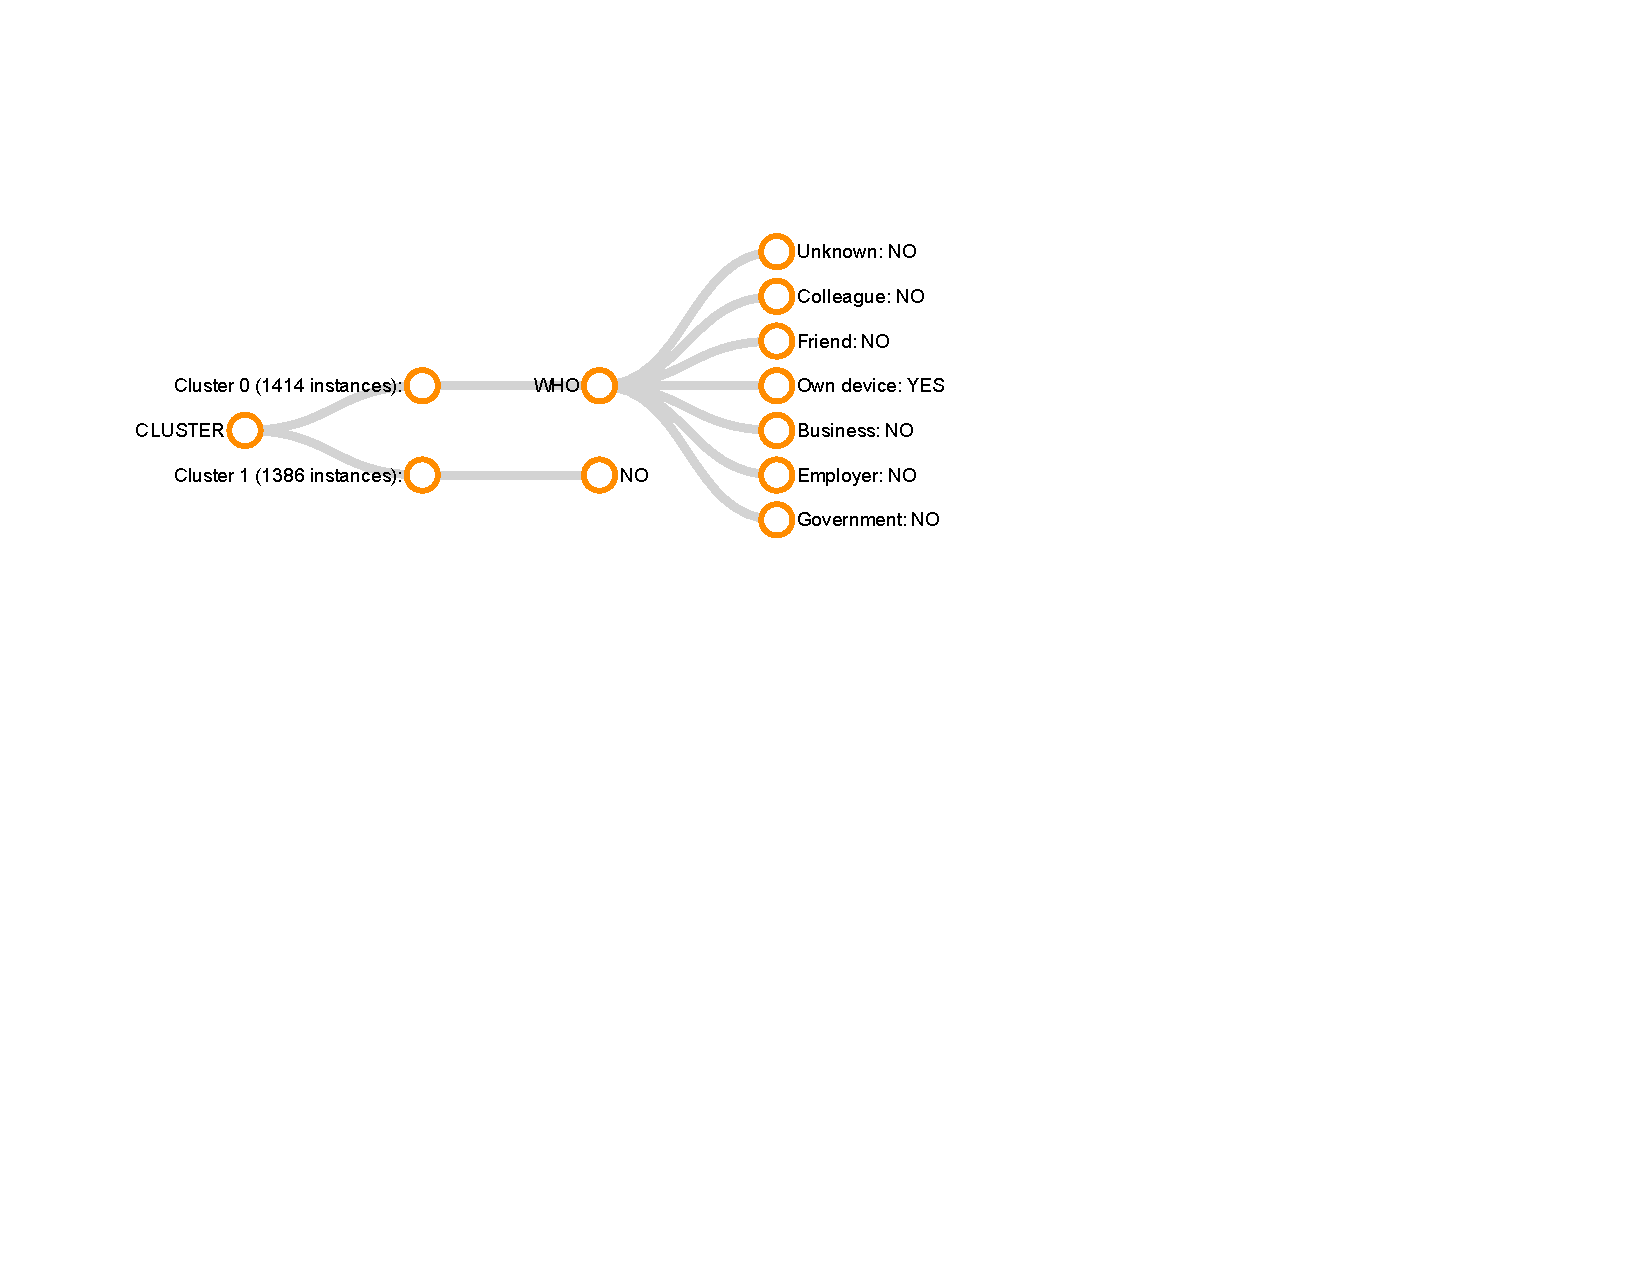
\includegraphics[width=0.48\textwidth]{figures/trait-based-2.pdf}
%	\caption{Trait-based clustering: 2-cluster tree}
%	\label{fig:2clustersAtd}
%\end{figure}




\subsection{Fit-based clustering}
Our fit-based clustering approach clusters participants without using any additional information. It instead uses the fit of the tree models to bootstrap the process of sorting participants into clusters. Like many bootstrapping methods, ours uses \emph{random starts} and \emph{iterative improvements} to find the optimal solution. The process is depicted in Figure~\ref{fig:flow_chart_fit}, and described in detail below. Accuracies of the resulting solutions are reported in Table~\ref{tab:comp_approach} under ``fit-based clustering''.

\begin{figure}[htp]
	\centering
	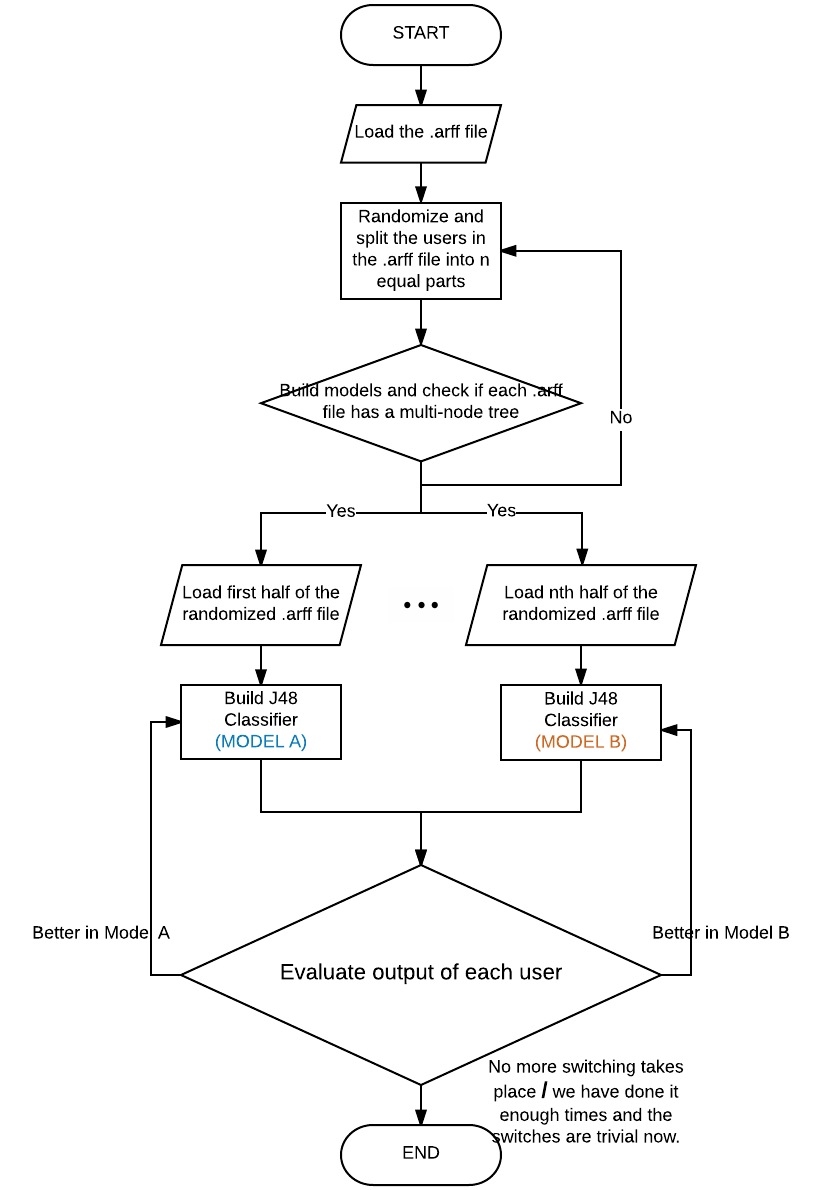
\includegraphics[width=0.8\textwidth]{figures/flowchartFit.png}
	\caption{The Flow Chart for Fit-based Clustering}
	\label{fig:flow_chart_fit}
\end{figure}

\textbf{Random starts:} We randomly divide particpants over $N$ separate groups, and learn a tree for each group. This is repeated until a non-trivial starting solution (i.e., with distinctly different trees per cluster) is found. 

\textbf{Iterative improvements:} Once each of the $N$ groups has a unique decision tree, we evaluate for each participant which of the trees best represents their 14 decisions. If this is the tree of a different group, we switch the participant to this group. Once all participants are evaluated and put in the group of their best-fitting tree, the tree in each group is re-learned with the data of the new group members. This then prompts another round of evaluations, and this process continues until no further switches are performed. 

Since this process is influenced by random chance, it is repeated in its entirety to find the optimal solution. Cross-validation is performed in the final step to prevent over-fitting. Accuracies of the 2- and 3-cluster solutions are reported in Table~\ref{tab:comp_approach} under ``fit-based clustering''. We were not able to converge on a higher number of clusters. 

The 2-cluster solution has a 77.99\% accuracy---a 6.7\% improvement over the ``smart default''. One profile has `no' for everything, while the settings in the other profile depends on \textbf{who}: it allows any collection by the user's `Own device', and may allow collection by a `Friend's device' or an `Employer', depending on \textbf{what} is collected.


%\begin{figure}
%	\centering
%	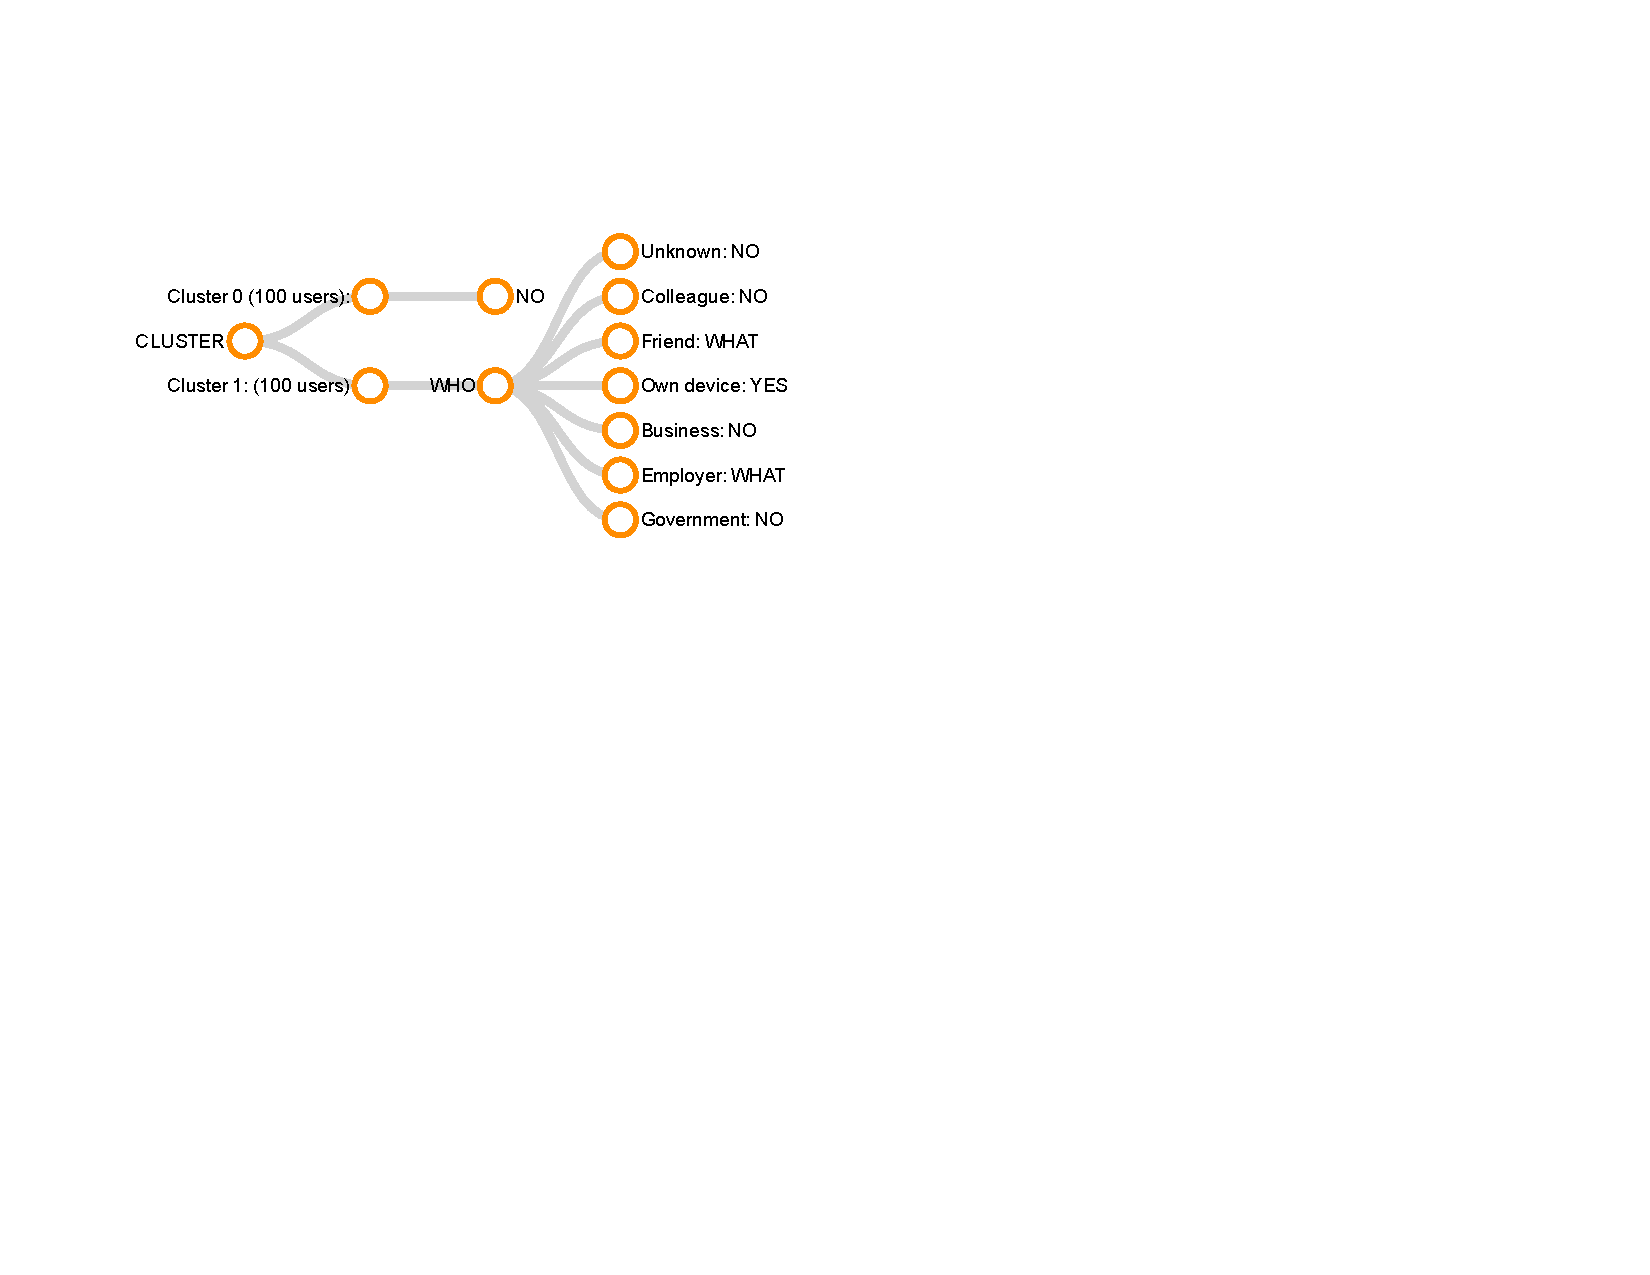
\includegraphics[width=.42\textwidth]{figures/fit-based-2c.pdf}
%	\caption{Fit-based clustering: 2-cluster tree. Further drill down for \textbf{who} = `Friend' or `Employer/School' in Cluster 1 is hidden for space reasons.}
%	\label{fig:2clustersFit}
%\end{figure}

The 3-cluster solution (Figure~\ref{fig:3clustersFit}) has a 81.54\% accuracy --- an 11.5\% improvement over the ``smart default''. We find one profile with `no' for everything; one profile that may allow collection by the user's `Own device', depending on \textbf{what} is being collected; and one profile that allows any collection except when the recipient (\textbf{who}) is `Unknown', the `Government', or a `Colleague', with settings for the latter depending on the \textbf{reason}.

\begin{figure*}
	\centering
	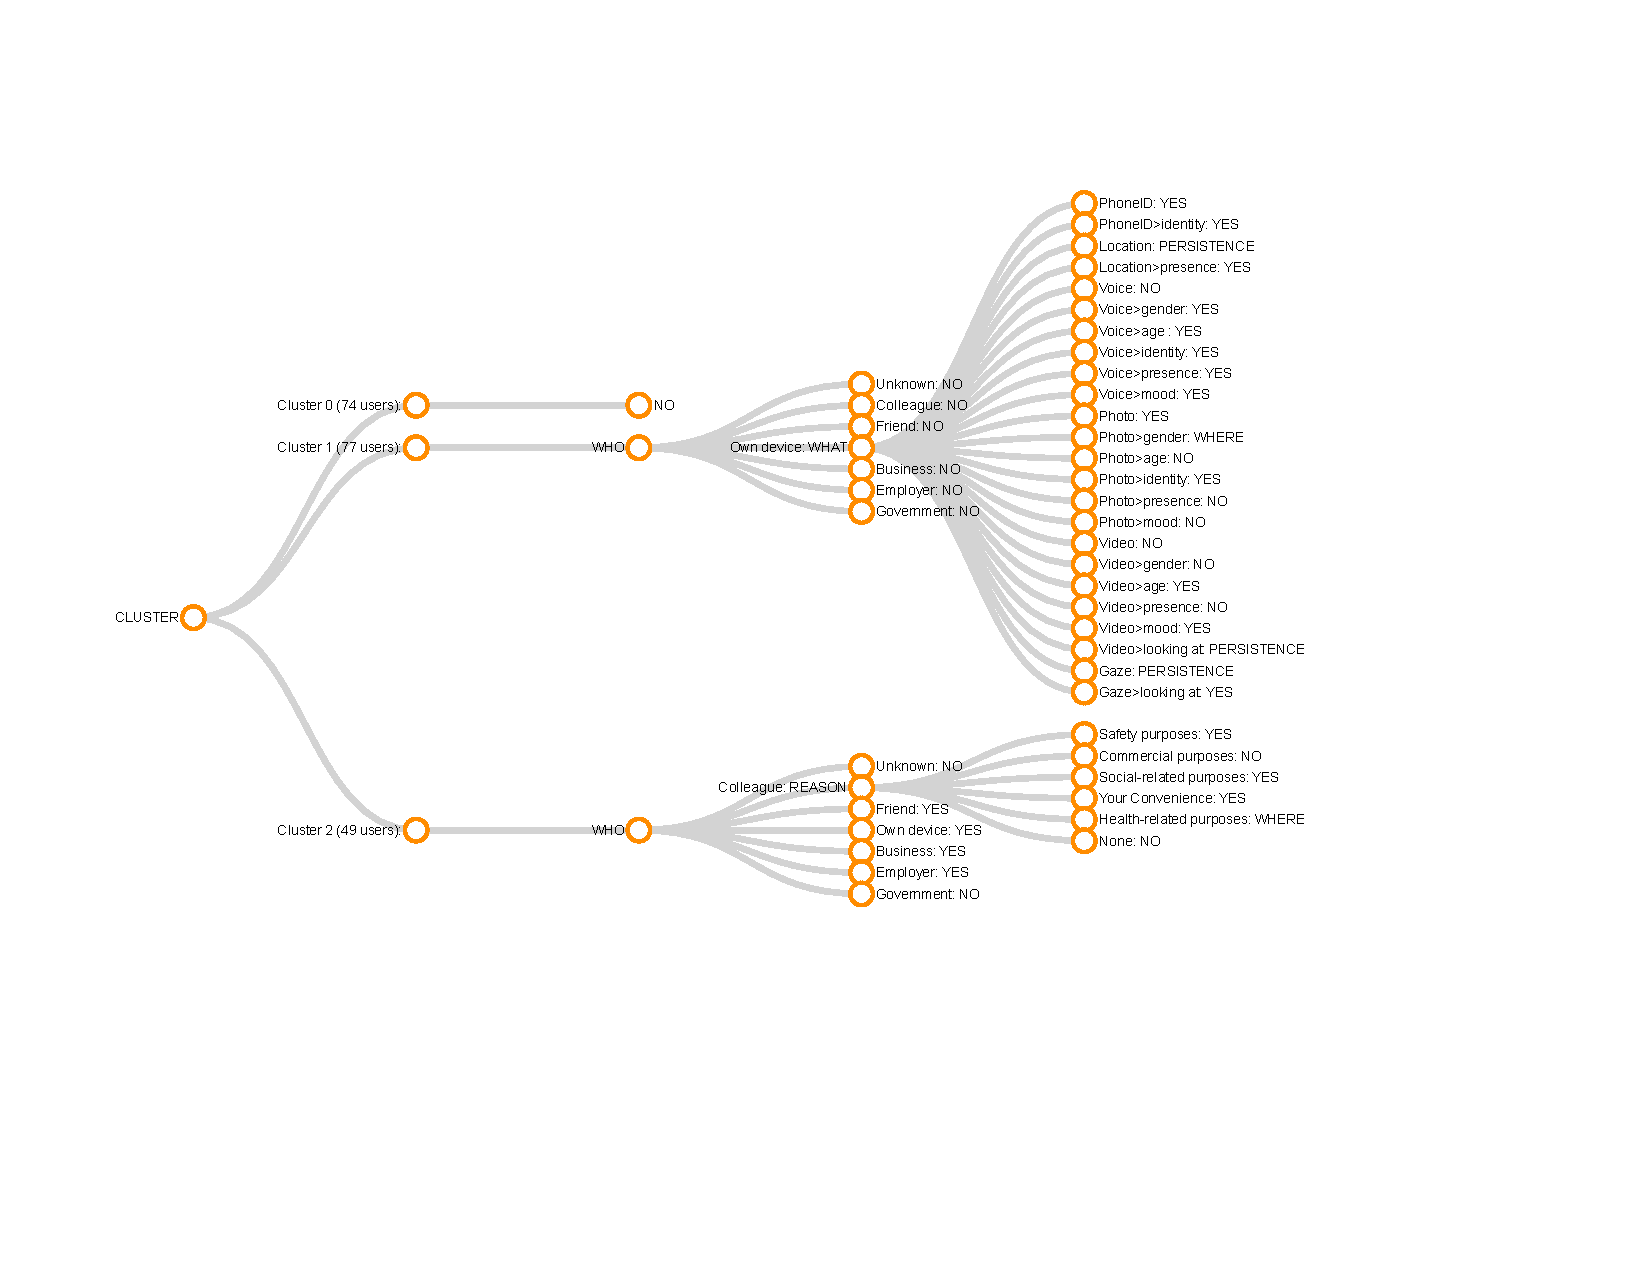
\includegraphics[width=\textwidth]{figures/fit-based-3c.pdf}
	\caption{Fit-based clustering: 3-cluster tree. Further drill down is hidden for space reasons.}
	\label{fig:3clustersFit}
\end{figure*}

\subsection{Agglomerative clustering}
Our final method for finding ``smart profiles'' follows a hierarchical bottom-up (or agglomerative) approach. It first fits a separate tree for each participant, and then iteratively merges them based on similarity. 156 of the initial 200 trees predict ``no for everything'' and 34 of them predict ``yes for everything''---these are merged first. For every possible pair of the remaining 10 trees, the accuracy of the pair is compared with the mean accuracy the individual trees, and the pair with the smallest reduction in accuracy is merged. This process is repeated until we reach the predefined number of clusters.

We were able to reach a 5- and 4-cluster solution. The 3-cluster solution collapsed down into a 2-cluster solution with one profile of all `yes'es and one profile of all `no's (a somewhat trivial solution with a relatively bad fit). Accuracies of the 4- and 5-cluster (Table~\ref{tab:comp_approach}, ``agglomerative clustering'') are 78.13\% and 78.27\% respectively. For the 4-cluster solution, we find one profile with `no' for everything, one profile with `yes' for everything, one profile that depends on \textbf{who}, and another that depends on \textbf{what}. The latter two profiles drill down even further on specific values of \textbf{who} and \textbf{what}, respectively.



\begin{figure}[t]
	\centering
	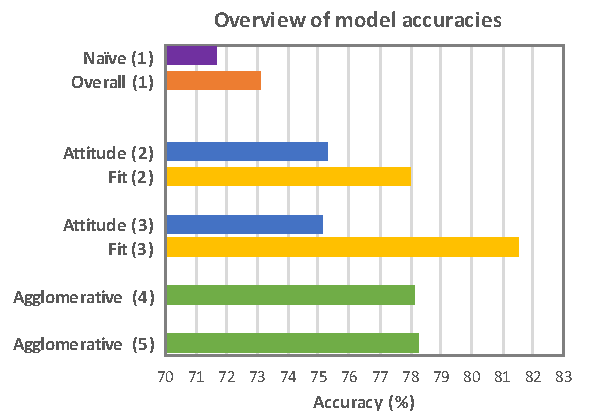
\includegraphics[width=0.43\textwidth]{figures/compare.pdf}
	\caption{Accuracy of our clustering approaches}
	\label{fig:comp_approach}
\end{figure}

\subsection{Discussion of Machine Learning Results}
Figure~\ref{fig:comp_approach} shows a comparison of the presented approaches. Compared to a naive default setting (all `no'), a ``smart default'' makes a 2.0\% improvement. The fit-based 2-cluster solution results in two ``smart profiles'' that make another 6.7\% improvement over the ``smart default'', while the three ``smart profiles'' of the fit-based 3-cluster solution make an 11.5\% improvement. If we let users choose the best option among these three profiles, they will on average be content with 81.54\% of the settings. This rivals the accuracy of some of the ``active tracking'' machine learning approaches~\cite{sadeh2009understanding}.

In line with our statistical results, the factor \textbf{who} seems to be the most prominent parameter, followed by \textbf{what}. In some cases the settings are more complex, depending on a combination of \textbf{who} and \textbf{what}. This is in line with the interaction effect observed in our statistical results.

Even our most accurate solution is not without fault, and its accuracy depends most on the \textbf{who} parameter. Specifically, the solution is most accurate for the user's own device, the device of a friend, and when the recipient is unknown. It is however less accurate when the recipient is a colleague, a nearby business, an employer, or the government. In these scenarios, more misclassifications tend to happen, so it would be useful to `guide' users to specifically have a look at these default settings, should they opt to make any manual overrides.

\section{Privacy-setting Prototypes (original work)}\label{sec:design1}
In Section~\ref{sec:sa1}, we developed a ``layered" interface that general IoT users can use to manually set their privacy settings (see Figure~\ref{fig:interface1}). Our machine learning analysis (Section~\ref{sec:predict1}) resulted in a number of interesting solutions for ``smart profiles'' that would allow users of this interface to set their privacy settings with a single click (i.e., a choice of profile). In this section we therefore present how we integrate the ``smart profiles" with our prototype. 

\subsection{Smart Default Setting}
The design of ``layered" interface is based on our statistical results that there exists no interaction effect between the parameters, our ``smart default" settings can be integrated to this prototype in nature. For ``yes to everything'' or ``no to everything'' default, we can just simply set all the settings in the Screen 4 of Figure~\ref{fig:interface1} to all `on' or `off'.

For the results from our Overall Prediction (see Figure~\ref{fig:naive_cls}), we can create a ``smart default'' setting that is 73.10\% accurate on average. In this version, the IoT settings for all devices are set to `off', except for `My own device', which will be set to the middle option. Table~\ref{tab:decisions} shows the default settings at deeper levels.
As this default setting is on average only 73.10\% accurate, we expect users to still change some of their settings. They can do this by navigating the manual settings interface.

\subsection{Smart Profiles}
To improve the accuracy of the default setting, we can instead build two ``smart profiles'', and allow the user to choose among them. Using the 3-cluster solution of the fit-based approach (see Figure~\ref{fig:3clustersFit}), we can attain an accuracy of 81.54\%. Screen 1 in Figure~\ref{fig:interface1} shows a selection screen where the user can choose between these profiles. The ``Limited collection'' profile allows the collection of any information by the user's own devices, their friends' devices, their employer/school's devices, and devices of nearby businesses. Devices of colleagues are only allowed to collect information for certain reasons. The ``Limited collection, personal devices only'' profile only allows the collection of certain types of information by the user's own devices. The ``No collection'' profile does not allow any data collection to take place by default.

Once the user chooses a profile, they will move to the manual settings interface (Screens 2--4), where they can further change some of their settings.

\begin{figure}[htb]
	\centering
	\begin{subfigure}[t]{0.24\textwidth}
		\centering
		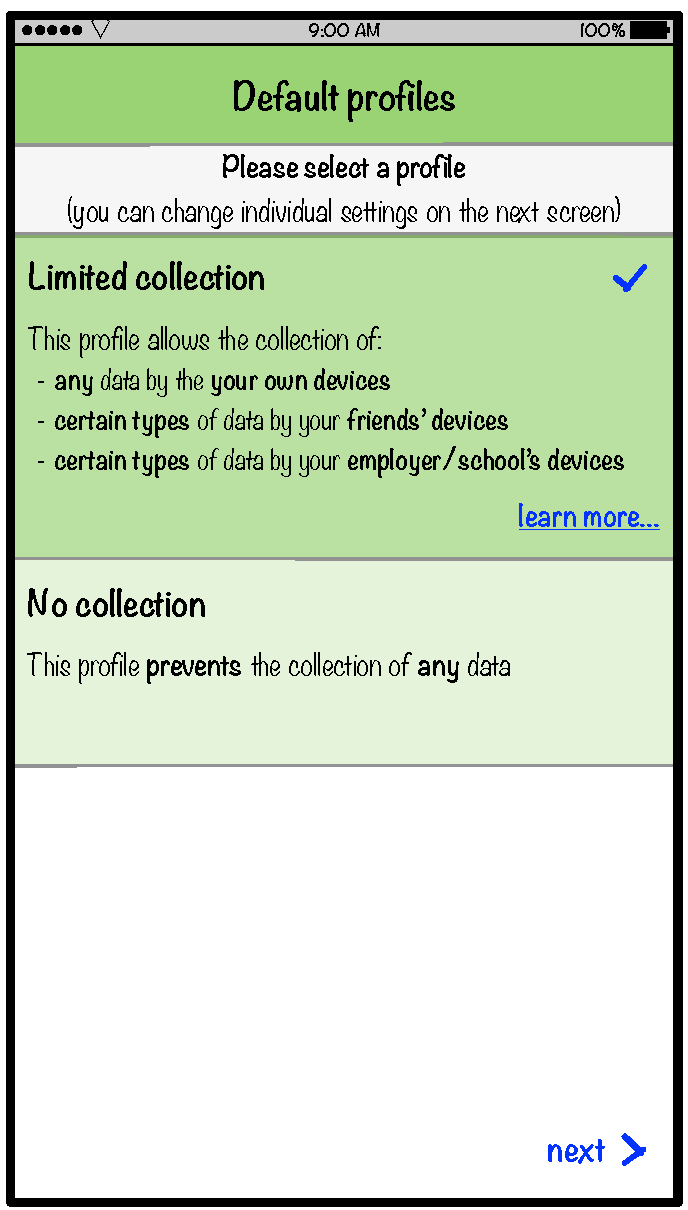
\includegraphics[height=2.8in]{figures/profiles2.pdf}
		\caption{2-profile choice interface}
		\label{fig:2profile_default_setting}
	\end{subfigure}%
	~~~~~~~~~
	\begin{subfigure}[t]{0.24\textwidth}
		\centering
		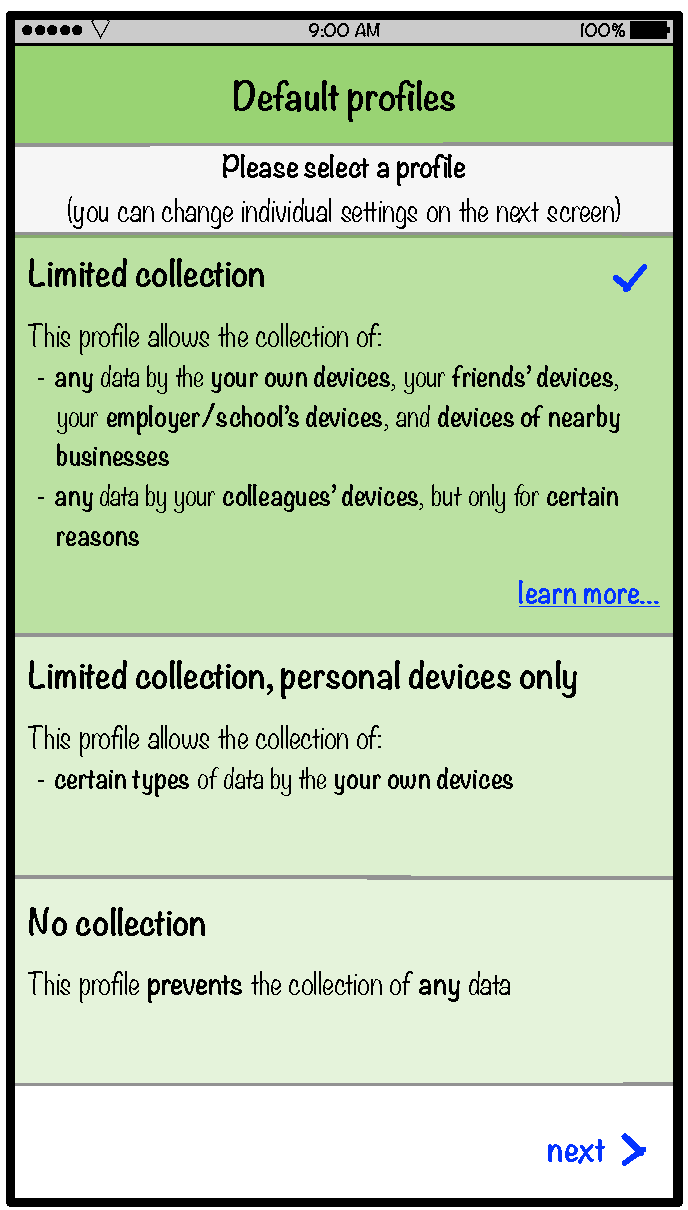
\includegraphics[height=2.8in]{figures/profiles3.pdf}
		\caption{3-profile choice interface}
		\label{fig:3profile_default_setting}
	\end{subfigure}%
	\caption{Two types of profile choice interfaces}
\end{figure}

\section{Summary}
In this chapter, we have presented the following:

\begin{itemize}
	\item Using statistical analysis, uncover the relative importance of the parameters that influence users' privacy decisions. Develop a ``layered interface'' in which these parameters are presented in decreasing order of importance.
	\item Using a tree-learning algorithm, create a decision tree that best predicts participants' choices based on the parameters. Use this tree to create a ``smart default'' setting.
	\item Using a combination of clustering and tree-learning algorithms, create a set of $N$ decision trees that best predict participants' choices. Use the trees to create $N$ ``smart profiles''.
	\item Develop a prototype for an IoT privacy-setting interface that integrates the layered interface with the smart default or the smart profiles.
\end{itemize}

Our statistical and machine learning results both indicated that recipient of the information (\textbf{who}) is the most significant parameter in users' decision to allow or reject IoT-based information collection. This parameter therefore features at the forefront in our layered settings interface, and plays an important role in our smart profiles. The \textbf{what} parameter was the second-most important decision parameter, and interacted significantly with the \textbf{who} parameter. This parameter therefore features at the second level of our settings interface, and further qualifies some of the settings in our smart profiles.

Our layered interface allows a further drill-down to the \textbf{reason} and \textbf{persistence} parameters, but given the relatively lesser importance of these parameters, we expect few users to engage with the interface at this level. Moreover, the \textbf{where} parameter was not significant, so we left it out of the interface.

While a naive (`no' to all) default setting in our interface would have provided an accuracy of 71.67\%, it would not have allowed users to reap the potential benefits associated with IoT data collection without changing the default setting. Our Overall Prediction procedure resulted in a smart default setting that was a bit more permissive, and increased the accuracy by 2\%.

The fit-based clustering approach, which iteratively clusters users and fits an optimal tree in each cluster, provided the best solution. This resulted in an interface where users can choose from 3 profiles, which increases the accuracy by another 11.5\%.

The scenario-based method presented in this paper is particularly suited for novel domains where few real interaction exist. We note, though, that this novelty may hamper our approach: users' decisions are inherently limited by the knowledge they have about IoT. Lee and Kobsa~\cite{lee2016understanding} made sure to educate users about the presented scenarios, hence their data is arguably better in this regard than data from ``live'' systems. However, as the adaptation of IoT becomes more widespread, the mindset and knowledge regarding such technologies---and thus their privacy preferences---might change. Our ``smart profiles'' may thus eventually have to be updated in future work, but for now, our current profiles can at least help users make make better privacy decisions in their initial stages of usage.

Our analysis allowed us to use \emph{data-driven design} to bootstrap the development of a privacy-setting interface, but a future user experiment could investigate whether users are comfortable with the layered interface, and whether they prefer a single ``smart default'' setting or a choice among ``smart profiles''.

In the next chapter, we discuss the challenges and solutions when we extended work that we have done in the domain of household IoT ("smart home") domain.
